\documentclass[a4paper,11pt]{scrartcl}

\usepackage{amsmath} % assumes amsmath package installed
\usepackage{amssymb}  % assumes amsmath package installed
\usepackage{amsfonts}
\usepackage{mathtools}
\usepackage{bbm}
\usepackage{bm}
\usepackage{color}
\usepackage{graphics} % for pdf, bitmapped graphics files
\usepackage{graphicx}
\usepackage{epsfig}   % for postscript graphics files
\usepackage{epstopdf}
\usepackage[noadjust]{cite} % basic fos bibliography [1]-[5]
\usepackage{tikz}
\usetikzlibrary{calc,positioning,shapes,shadows,arrows,fit}
\usepackage{fancyhdr}
\usepackage{framed}
\usepackage{float}
\usepackage{comment}
                               % symboler.
\usepackage[latin1]{inputenc}  % Ser till s� att svenska tecken
                               % fungerar.
%\usepackage[swedish]{babel}    % LaTeX t�nker svenskt.

%\addtolength{\topmargin}{-20mm}% Drar bort 20mm fr�n topmarginalen
                               % kommentera bort raden om du �r n�jd
                               % med avst�ndet. Det finns fler
                               % parametrar att justera om du inte f�r
                               % plats p� de utsatta antalet sidor.
%\addtolength{\textheight}{20mm}% Det vi drog bort fr�n topmarginalen
                               % l�gger vi till i texth�jden.

\usepackage{fancyhdr}
\usepackage{lastpage}
\usepackage{listings}
\usepackage{hyperref}

%\pagestyle{fancy}
%\usepackage{hyperref} %[colorlinks]
%\usepackage[figure,table]{hypcap}



%%%%%%%%%%%%%%%%%%%%%%%%%%%%%%%%%%%%%%%%%%%%%

\begin{document}


\begin{figure}[ht!]
	\centering
	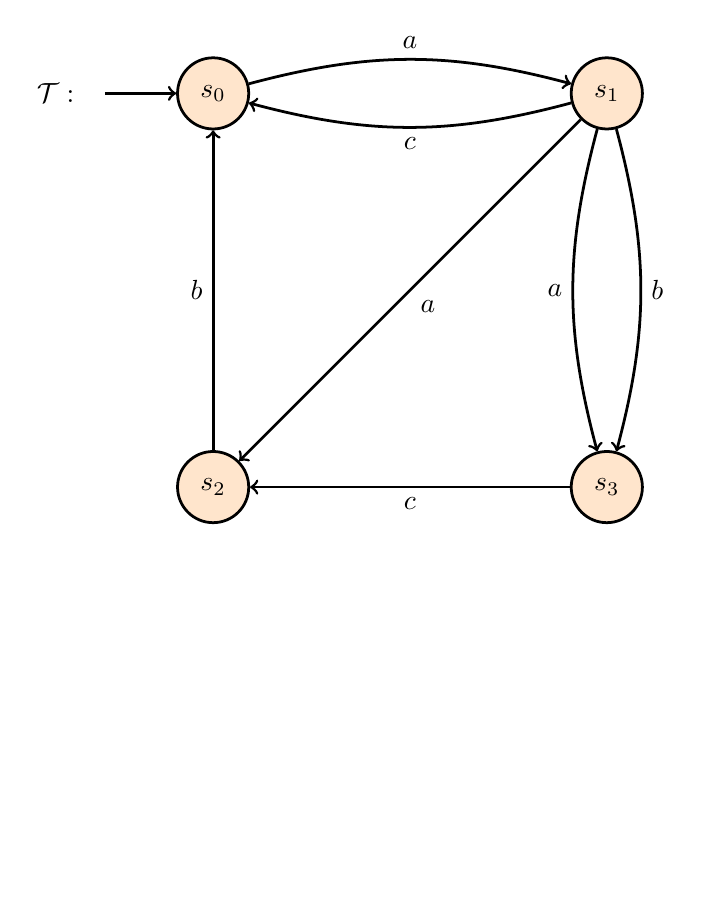
\begin{tikzpicture}[scale = 1.0]     
	\node(pseudo1) at (-1.5,0){};
	\node(pseudo2) at (-1.5,-10){};
	\node(0) [line width = 1.0] at (0,0)[shape=circle,draw][fill=orange!20] {$\ s_0 \ $};
	\node(1) [line width = 1.0] at (5.0,0)[shape=circle,draw][fill=orange!20] {$\ s_1 \ $};
	\node [align = center, line width = 1.0] (2) at (0.0,-5.0)[shape=circle,draw][fill=orange!20] {$\ s_2 \ $};
	\node [align = center, line width = 1.0] (3) at (5.0,-5.0)[shape=circle,draw][fill=orange!20] {$\ s_3 \ $};
	
	
	\path [->] [line width = 1.0]
	(0) edge [bend left = 15] node [above]      {$a$}   (1)
	(2) edge [bend right = 0] node [left]      {$b$}   (0)
	(1) edge [bend left = 15] node [below]      {$c$} (0)
	(1) edge                  node [below right] {$a$} (2)
	(1) edge [bend right = 15] node [left] {$a$}  (3)
	(1) edge [bend left = 15] node [right] {$b$}  (3)
	(3) edge node [below] {$c$}  (2)
	(pseudo1) edge                                   (0);
	
	\node at (-2,0) {$\mathcal{T}: $};
	\end{tikzpicture}
	\caption{The Transition Systems $\mathcal{T}$.}
	\label{fig:transition_systems}
\end{figure}

\end{document}
